\documentclass[a4paper,12pt]{article} 

% First, we usually want to set the margins of our document. For this we use the package geometry.
\usepackage[top = 2.5cm, bottom = 2.5cm, left = 2.5cm, right = 2.5cm]{geometry} 
\usepackage[T1]{fontenc}
\usepackage[utf8]{inputenc}

% The following two packages - multirow and booktabs - are needed to create nice looking tables.
\usepackage{multirow} % Multirow is for tables with multiple rows within one cell.
\usepackage{booktabs} % For even nicer tables.

% As we usually want to include some plots (.pdf files) we need a package for that.
\usepackage{graphicx} 

% The default setting of LaTeX is to indent new paragraphs. This is useful for articles. But not really nice for homework problem sets. The following command sets the indent to 0.
\usepackage{setspace}
\setlength{\parindent}{0in}

% Package to place figures where you want them.
\usepackage{float}

% The fancyhdr package let's us create nice headers.
\usepackage{fancyhdr}

\usepackage{amsmath,amsthm,tikz}

% To make our document nice we want a header and number the pages in the footer.

\pagestyle{fancy} % With this command we can customize the header style.

\fancyhf{} % This makes sure we do not have other information in our header or footer.

\lhead{\footnotesize Data Structure and Algorithm Analysis(H): Work Sheet 13}% \lhead puts text in the top left corner. \footnotesize sets our font to a smaller size.

%\rhead works just like \lhead (you can also use \chead)
\rhead{\footnotesize Mengxuan Wu} %<---- Fill in your lastnames.

% Similar commands work for the footer (\lfoot, \cfoot and \rfoot).
% We want to put our page number in the center.
\cfoot{\footnotesize \thepage} 

\begin{document}

\thispagestyle{empty} % This command disables the header on the first page. 

\begin{tabular}{p{15.5cm}}
{\large \bf Data Structure and Algorithm Analysis(H)} \\
Southern University of Science and Technology \\ Mengxuan Wu \\ 12212006 \\
\hline
\\
\end{tabular}

\vspace*{0.3cm} %add some vertical space in between the line and our title.

\begin{center}
	{\Large \bf Work Sheet 13}
	\vspace{2mm}

	{\bf Mengxuan Wu}
		
\end{center}  

\vspace{0.4cm}

\section*{Question 13.1}

\subsection*{1.}

To find the in-degree of one vertex with adjacency list, we need to traverse the whole list to find the vertex. 
So the time complexity is $O(|V|+|E|)$.

\subsection*{2.}

To find the in-degree of all vertices with adjacency list, we need to traverse the whole list to find the vertex.
So the time complexity is $O(|V|+|E|)$.

\subsection*{3.}

To find the in-degree of one vertex with adjacency matrix, we need to traverse one column of the matrix.
So the time complexity is $O(|V|)$.

\subsection*{4.}

To find the in-degree of all vertices with adjacency matrix, we need to traverse all columns of the matrix.
So the time complexity is $O(|V|^2)$.

\section*{Question 13.2}

The mayor's strategy is not always optimal.
Consider the graph that all the vertices are connected to each other.
Then the mayor's strategy will put two cameras on two vertices, while the optimal strategy is to put one camera on one vertex.

However, this strategy sometimes can be optimal.
Consider a triangle shape graph with 3 vertices and 3 edges.
Then the mayor's strategy will put two cameras, which is optimal.

The mayor's strategy's efficiency mainly depends on the shape of the graph.
If there are many loops with odd number of vertices, then the mayor's strategy will be good, since in an odd loop there must be one edge that has cameras on both ends.

The greedy strategy for this problem is that put cameras on the vertices that have the most unmonitored edges.
\section*{Question 13.3}

\begin{figure}[H]
	\begin{minipage}{0.5\linewidth}
		\centering
		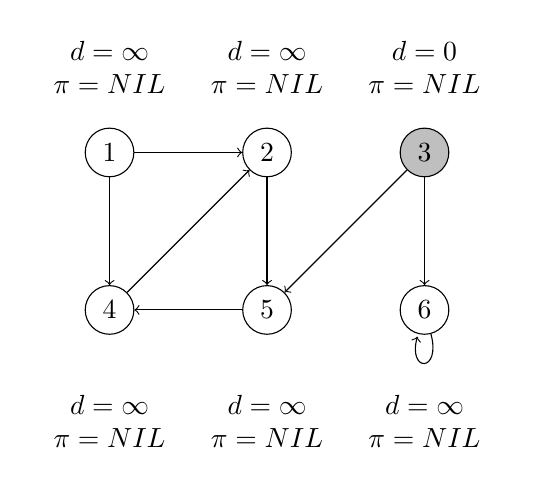
\begin{tikzpicture}
			\draw (0,0) node [circle,draw] (1) {1};
			\draw (0,0.5) node [above] {\begin{tabular}{c} $d = \infty$ \\ $\pi = NIL$ \end{tabular}};
			\draw (2,0) node [circle,draw] (2) {2};
			\draw (2,0.5) node [above] {\begin{tabular}{c} $d = \infty$ \\ $\pi = NIL$ \end{tabular}};
			\draw (4,0) node [circle,draw,fill=black!25] (3) {3};
			\draw (4,0.5) node [above] {\begin{tabular}{c} $d = 0$ \\ $\pi = NIL$ \end{tabular}};
			\draw (0,-2) node [circle,draw] (4) {4};
			\draw (0,-4) node [above] {\begin{tabular}{c} $d = \infty$ \\ $\pi = NIL$ \end{tabular}};
			\draw (2,-2) node [circle,draw] (5) {5};
			\draw (2,-4) node [above] {\begin{tabular}{c} $d = \infty$ \\ $\pi = NIL$ \end{tabular}};
			\draw (4,-2) node [circle,draw] (6) {6};
			\draw (4,-4) node [above] {\begin{tabular}{c} $d = \infty$ \\ $\pi = NIL$ \end{tabular}};
			\path[->]
				(1) edge (2)
					edge (4)
				(2) edge (5)
				(3) edge (5)
					edge (6)
				(4) edge (2)
				(5) edge (4)
				(6) edge [loop below] (6);
		\end{tikzpicture}
	\end{minipage}
	\begin{minipage}{0.5\linewidth}
		\centering
		\begin{tabular}{|c|}
			\hline
			3 \\ \hline
		\end{tabular}

		\begin{tabular}{c}
			0
		\end{tabular}
	\end{minipage}
\end{figure}

\begin{figure}[H]
	\begin{minipage}{0.5\linewidth}
		\centering
		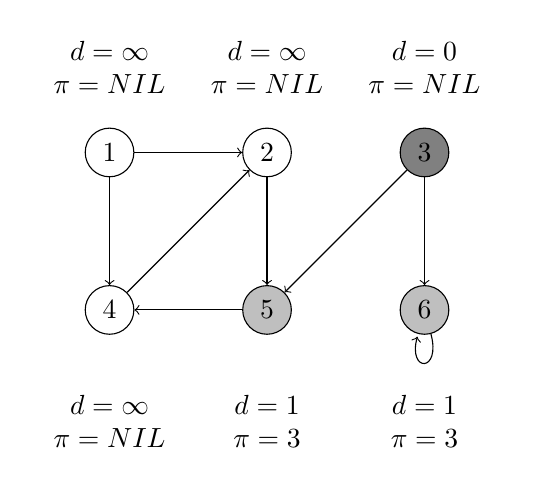
\begin{tikzpicture}
			\draw (0,0) node [circle,draw] (1) {1};
			\draw (0,0.5) node [above] {\begin{tabular}{c} $d = \infty$ \\ $\pi = NIL$ \end{tabular}};
			\draw (2,0) node [circle,draw] (2) {2};
			\draw (2,0.5) node [above] {\begin{tabular}{c} $d = \infty$ \\ $\pi = NIL$ \end{tabular}};
			\draw (4,0) node [circle,draw,fill=black!50] (3) {3};
			\draw (4,0.5) node [above] {\begin{tabular}{c} $d = 0$ \\ $\pi = NIL$ \end{tabular}};
			\draw (0,-2) node [circle,draw] (4) {4};
			\draw (0,-4) node [above] {\begin{tabular}{c} $d = \infty$ \\ $\pi = NIL$ \end{tabular}};
			\draw (2,-2) node [circle,draw,fill=black!25] (5) {5};
			\draw (2,-4) node [above] {\begin{tabular}{c} $d = 1$ \\ $\pi = 3$ \end{tabular}};
			\draw (4,-2) node [circle,draw,fill=black!25] (6) {6};
			\draw (4,-4) node [above] {\begin{tabular}{c} $d = 1$ \\ $\pi = 3$ \end{tabular}};
			\path[->]
				(1) edge (2)
					edge (4)
				(2) edge (5)
				(3) edge (5)
					edge (6)
				(4) edge (2)
				(5) edge (4)
				(6) edge [loop below] (6);
		\end{tikzpicture}
	\end{minipage}
	\begin{minipage}{0.5\linewidth}
		\centering
		\begin{tabular}{|c|c|}
			\hline
			5 & 6 \\ \hline
		\end{tabular}

		\begin{tabular}{cc}
			1 & 1
		\end{tabular}
	\end{minipage}
\end{figure}

\begin{figure}[H]
	\begin{minipage}{0.5\linewidth}
		\centering
		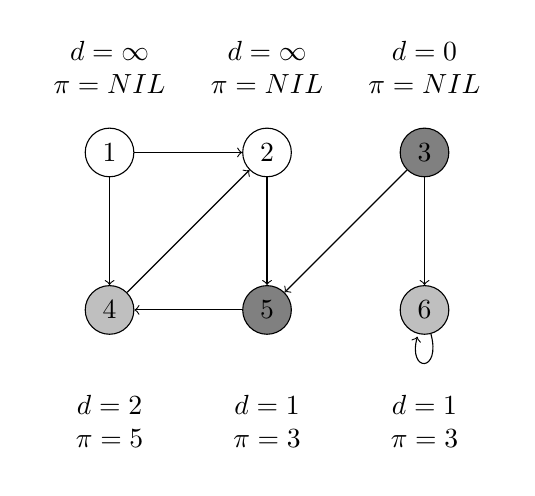
\begin{tikzpicture}
			\draw (0,0) node [circle,draw] (1) {1};
			\draw (0,0.5) node [above] {\begin{tabular}{c} $d = \infty$ \\ $\pi = NIL$ \end{tabular}};
			\draw (2,0) node [circle,draw] (2) {2};
			\draw (2,0.5) node [above] {\begin{tabular}{c} $d = \infty$ \\ $\pi = NIL$ \end{tabular}};
			\draw (4,0) node [circle,draw,fill=black!50] (3) {3};
			\draw (4,0.5) node [above] {\begin{tabular}{c} $d = 0$ \\ $\pi = NIL$ \end{tabular}};
			\draw (0,-2) node [circle,draw,fill=black!25] (4) {4};
			\draw (0,-4) node [above] {\begin{tabular}{c} $d = 2$ \\ $\pi = 5$ \end{tabular}};
			\draw (2,-2) node [circle,draw,fill=black!50] (5) {5};
			\draw (2,-4) node [above] {\begin{tabular}{c} $d = 1$ \\ $\pi = 3$ \end{tabular}};
			\draw (4,-2) node [circle,draw,fill=black!25] (6) {6};
			\draw (4,-4) node [above] {\begin{tabular}{c} $d = 1$ \\ $\pi = 3$ \end{tabular}};
			\path[->]
				(1) edge (2)
					edge (4)
				(2) edge (5)
				(3) edge (5)
					edge (6)
				(4) edge (2)
				(5) edge (4)
				(6) edge [loop below] (6);
		\end{tikzpicture}
	\end{minipage}
	\begin{minipage}{0.5\linewidth}
		\centering
		\begin{tabular}{|c|c|}
			\hline
			6 & 4 \\ \hline
		\end{tabular}

		\begin{tabular}{cc}
			1 & 2
		\end{tabular}
	\end{minipage}
\end{figure}

\begin{figure}[H]
	\begin{minipage}{0.5\linewidth}
		\centering
		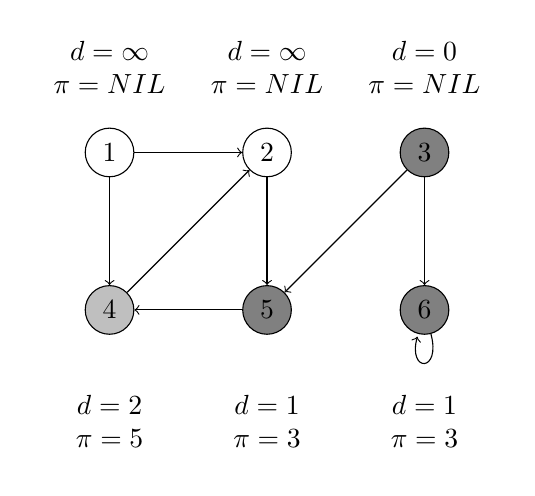
\begin{tikzpicture}
			\draw (0,0) node [circle,draw] (1) {1};
			\draw (0,0.5) node [above] {\begin{tabular}{c} $d = \infty$ \\ $\pi = NIL$ \end{tabular}};
			\draw (2,0) node [circle,draw] (2) {2};
			\draw (2,0.5) node [above] {\begin{tabular}{c} $d = \infty$ \\ $\pi = NIL$ \end{tabular}};
			\draw (4,0) node [circle,draw,fill=black!50] (3) {3};
			\draw (4,0.5) node [above] {\begin{tabular}{c} $d = 0$ \\ $\pi = NIL$ \end{tabular}};
			\draw (0,-2) node [circle,draw,fill=black!25] (4) {4};
			\draw (0,-4) node [above] {\begin{tabular}{c} $d = 2$ \\ $\pi = 5$ \end{tabular}};
			\draw (2,-2) node [circle,draw,fill=black!50] (5) {5};
			\draw (2,-4) node [above] {\begin{tabular}{c} $d = 1$ \\ $\pi = 3$ \end{tabular}};
			\draw (4,-2) node [circle,draw,fill=black!50] (6) {6};
			\draw (4,-4) node [above] {\begin{tabular}{c} $d = 1$ \\ $\pi = 3$ \end{tabular}};
			\path[->]
				(1) edge (2)
					edge (4)
				(2) edge (5)
				(3) edge (5)
					edge (6)
				(4) edge (2)
				(5) edge (4)
				(6) edge [loop below] (6);
		\end{tikzpicture}
	\end{minipage}
	\begin{minipage}{0.5\linewidth}
		\centering
		\begin{tabular}{|c|}
			\hline
			4 \\ \hline
		\end{tabular}

		\begin{tabular}{cc}
			2
		\end{tabular}
	\end{minipage}
\end{figure}

\begin{figure}[H]
	\begin{minipage}{0.5\linewidth}
		\centering
		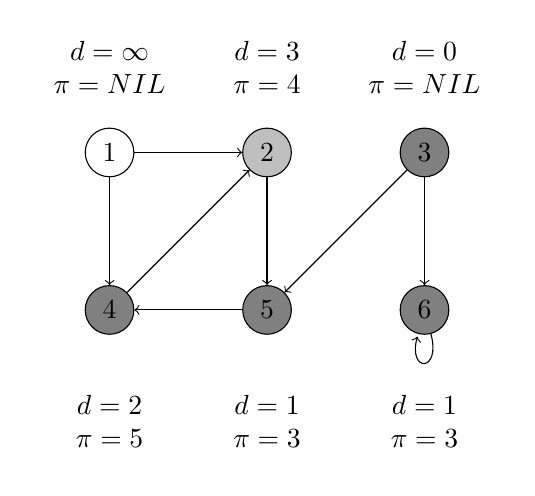
\begin{tikzpicture}
			\draw (0,0) node [circle,draw] (1) {1};
			\draw (0,0.5) node [above] {\begin{tabular}{c} $d = \infty$ \\ $\pi = NIL$ \end{tabular}};
			\draw (2,0) node [circle,draw,fill=black!25] (2) {2};
			\draw (2,0.5) node [above] {\begin{tabular}{c} $d = 3$ \\ $\pi = 4$ \end{tabular}};
			\draw (4,0) node [circle,draw,fill=black!50] (3) {3};
			\draw (4,0.5) node [above] {\begin{tabular}{c} $d = 0$ \\ $\pi = NIL$ \end{tabular}};
			\draw (0,-2) node [circle,draw,fill=black!50] (4) {4};
			\draw (0,-4) node [above] {\begin{tabular}{c} $d = 2$ \\ $\pi = 5$ \end{tabular}};
			\draw (2,-2) node [circle,draw,fill=black!50] (5) {5};
			\draw (2,-4) node [above] {\begin{tabular}{c} $d = 1$ \\ $\pi = 3$ \end{tabular}};
			\draw (4,-2) node [circle,draw,fill=black!50] (6) {6};
			\draw (4,-4) node [above] {\begin{tabular}{c} $d = 1$ \\ $\pi = 3$ \end{tabular}};
			\path[->]
				(1) edge (2)
					edge (4)
				(2) edge (5)
				(3) edge (5)
					edge (6)
				(4) edge (2)
				(5) edge (4)
				(6) edge [loop below] (6);
		\end{tikzpicture}
	\end{minipage}
	\begin{minipage}{0.5\linewidth}
		\centering
		\begin{tabular}{|c|}
			\hline
			2 \\ \hline
		\end{tabular}

		\begin{tabular}{cc}
			3
		\end{tabular}
	\end{minipage}
\end{figure}

\begin{figure}[H]
	\begin{minipage}{0.5\linewidth}
		\centering
		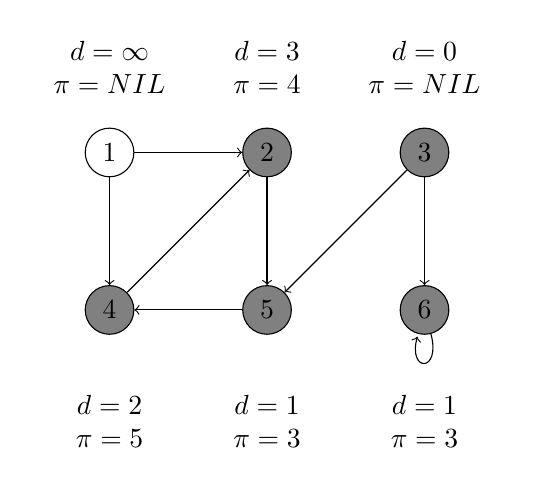
\begin{tikzpicture}
			\draw (0,0) node [circle,draw] (1) {1};
			\draw (0,0.5) node [above] {\begin{tabular}{c} $d = \infty$ \\ $\pi = NIL$ \end{tabular}};
			\draw (2,0) node [circle,draw,fill=black!50] (2) {2};
			\draw (2,0.5) node [above] {\begin{tabular}{c} $d = 3$ \\ $\pi = 4$ \end{tabular}};
			\draw (4,0) node [circle,draw,fill=black!50] (3) {3};
			\draw (4,0.5) node [above] {\begin{tabular}{c} $d = 0$ \\ $\pi = NIL$ \end{tabular}};
			\draw (0,-2) node [circle,draw,fill=black!50] (4) {4};
			\draw (0,-4) node [above] {\begin{tabular}{c} $d = 2$ \\ $\pi = 5$ \end{tabular}};
			\draw (2,-2) node [circle,draw,fill=black!50] (5) {5};
			\draw (2,-4) node [above] {\begin{tabular}{c} $d = 1$ \\ $\pi = 3$ \end{tabular}};
			\draw (4,-2) node [circle,draw,fill=black!50] (6) {6};
			\draw (4,-4) node [above] {\begin{tabular}{c} $d = 1$ \\ $\pi = 3$ \end{tabular}};
			\path[->]
				(1) edge (2)
					edge (4)
				(2) edge (5)
				(3) edge (5)
					edge (6)
				(4) edge (2)
				(5) edge (4)
				(6) edge [loop below] (6);
		\end{tikzpicture}
	\end{minipage}
	\begin{minipage}{0.5\linewidth}
		\centering
		\begin{tabular}{c}
			$\emptyset$
		\end{tabular}
	\end{minipage}
\end{figure}


\section*{Question 13.4}

If we use 1 bit to store color in BFS, there is no difference with current implementation.
However, we do lose the information of whether the vertex is processed or not.

\section*{Question 13.5}

If we use adjacency matrix to implement BFS, we need to traverse the whole row to find the adjacent vertices.
And since we need to traverse all vertices, the time complexity is $O(|V| \times |V|) = O(|V|^2)$.
\end{document}